\chapter{Recuperaci\'on de Imágenes}\label{chapter:ImIp} % II = Image Inpainting

\begin{definition}
El problema de \II, o en general el problema de \textit{inpainting} es el de recuperar una señal a partir de una versi\'on corrupta de la misma. Sea $\y$ un vector de dimensiones $m \times 1$ y $\z$ la versi\'on corrupta de $\y$ que le faltan algunos elementos, se tiene que:
\begin{equation}
	z = My
	\label{eq:inpainting}
\end{equation}
donde $\mathbf{M}$ es una matriz diagonal de $m \times m$ con solo $0$'s y $1$'s la cual define las posiciones de los elementos faltantes. Se quiere encontrar el vector $\y$, cuando $\z$ y  $\mathbf{M}$ son conocidos. 
\end{definition}

Se ha de destacar que estamos en presencia de un problema mal planteado pues la $y$ buscada que satisface \ref{eq:inpainting} hay mas de una (en el caso del problema general sin restricciones hay infinitas). Entre las dis\'imiles soluciones se busca la que bajo criterios subjetivos del ojo humano es la que mejor rellena las partes faltantes. 

\section{Los parches de una imagen}\label{sec:patches}

\begin{definition}
	Un parche  de una imagen (matriz) dada no es m\'as que una subimagen (submatriz) cuadrada de dimensiones $\sqrt{n} \times \sqrt{n}$. El tamaño del parche es $n$ y usualmente es muy peque\~no comparado con las dimensiones de la imagen.
\end{definition}

\begin{figure}[h]
	\centering
	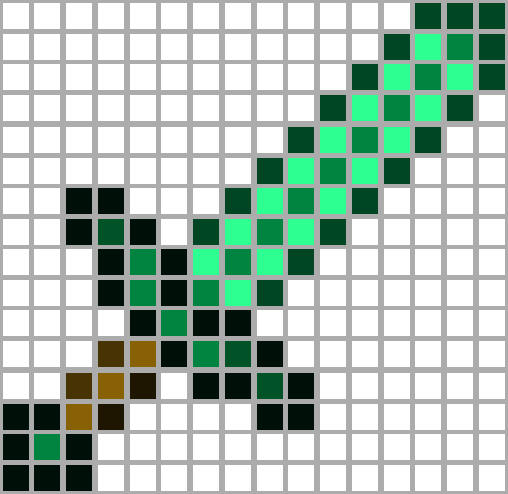
\includegraphics[width=4cm, height=4cm]{Graphics/diamon_sword.png}
	\hspace{1cm}
	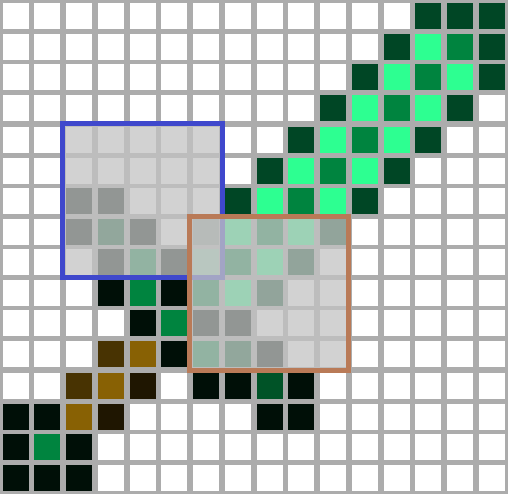
\includegraphics[width=4cm, height=4cm]{Graphics/diamon_sword_with_patches.png}
	\caption{Una imagen de $16 \times 16$ y dos parches de esta tomando $n = 25$.}
	\label{ex:patches}
\end{figure}

En la figura \ref{ex:patches} se ejemplifica visualmente el concepto de parches. Como vemos estos pueden solaparse sin ning\'un problema. Es de inter\'es en el siguiente cap\'itulo el conjunto de todos los parches, incluyendo con solapamientos.

\begin{lemma}\label{le:count_patches}
	La cantidad de parches de una matriz (imagen) incluyendo los solapamientos, para una matriz $A$ de dimensiones $a \times b$, y tomando los parches de $\sqrt{n} \times \sqrt{n}$, es igual a:
	
	\begin{equation}
		(a - \sqrt{n} + 1)(b - \sqrt{n} + 1)
		\label{eq:count_patches}
	\end{equation}
\end{lemma}


\textbf{Demostraci\'on:} tomando como referencia la esquina superior izquierda de un parche, esta solo puede ser ubicada verticalmente en el intervalo de posiciones \\$[1,\; a - \sqrt{n} + 1]$, de lo contrario el parche sobresaldr\'ia de la imagen. An\'alogamente solo puede ser colocado horizontalmente en el intervalo de posiciones $[1,\; b - \sqrt{n} + 1]$. Aplicando el principio combinatorio de la multiplicaci\'on, un parche puede ser ubicado de $(a - \sqrt{n} + 1)(b - \sqrt{n} + 1)$ formas distintas $\blacksquare$.

\begin{lemma}\label{le:count_patches_ieq}
	La cantidad de parches con solapamiento de una matriz A, con $n > 1$, es menor que la cantidad de elementos de la misma.
\end{lemma}

\textbf{Demostraci\'on:} Sea $A$ de $a \times b$; dado que $n > 1$ se cumple la siguiente desigualdad:

\begin{equation}
	\begin{array}{lrcl}
		                &               1 &<& n        \\ 
		\Longrightarrow &               1 &<& \sqrt{n} \\
		\Longrightarrow &   -\sqrt{n} + 1 &<& 0        \\
		\Longrightarrow & a -\sqrt{n} + 1 &<& a        \\
	\end{array}
\end{equation}

An\'alogamente $b -\sqrt{n} + 1 < b$, multiplicando las dos desigualdades obtenemos:

\begin{equation}
	(a - \sqrt{n} + 1)(b - \sqrt{n} + 1) < ab
	\label{eq:count_patches_ieq}
\end{equation}

Por el lema \ref{le:count_patches} la cantidad de parches de A es $(a - \sqrt{n} + 1)(b - \sqrt{n} + 1)$ lo que es menor que $ab$ $\blacksquare$.

\begin{definition}
	El p\'ixel o elemento central de un parche es aquel que se encuentra en una posici\'on prefijada, dicha posici\'on debe ser la misma para todos los parches de una misma imagen.
\end{definition}

\begin{figure}[h]
	\centering
	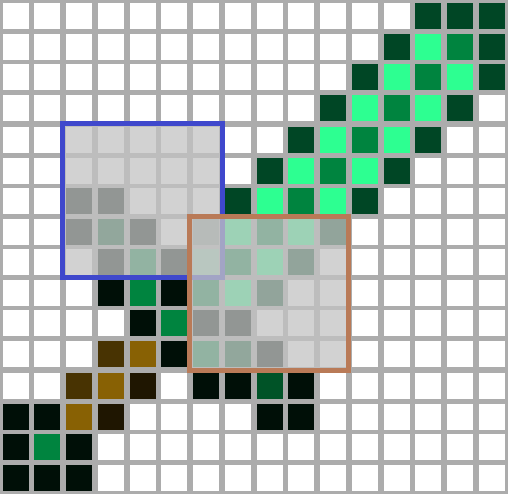
\includegraphics[width=4cm, height=4cm]{Graphics/diamon_sword_with_patches.png}
	\hspace{1cm}
	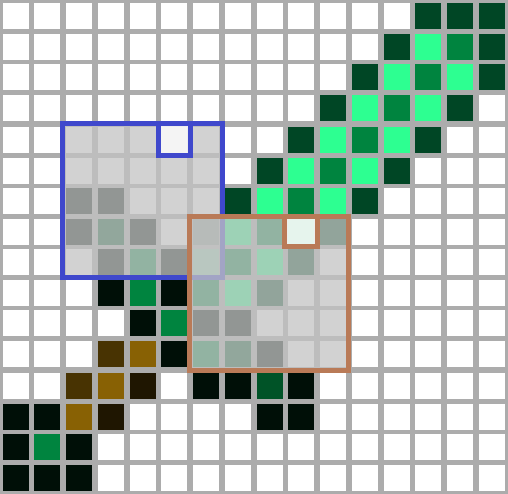
\includegraphics[width=4cm, height=4cm]{Graphics/diamon_sword_with_patches_and_centers.png}
	\caption{Parches con p\'ixel central (marcado en rojo) situado en la posici\'on $4$.}
	\label{ex:patch_center}
\end{figure}

En la figura \ref{ex:patch_center} se muestran los centros de los parches del ejemplo anterior. No debemos confundir el p\'ixel central con aquel que se encuentra en su centro geom\'etrico. La idea de este elemento es para tomarlo como punto de referencia o representativo. Un ejemplo se ve en el cap\'itulo \ref{chapter:SCHEME}, como para aquellos p\'ixles que no se conoce su valor, se usa en cambio el parche del cual ellos son su centro.